\documentclass{book}
\usepackage[T1]{fontenc}
\usepackage{tikz}
\usepackage{verbatim}
\usetikzlibrary{shapes}
\usepackage{amsmath}
\usepackage{xspace}

\usepackage{graphicx,txfonts,color,xspace,cite,url}
\usepackage[colorlinks=true,pdfborder={0,0,0}]{hyperref}
\usepackage[backgroundcolor=orange!20,bordercolor=orange,textsize=small]{todonotes}


%latex2html hack
\pagecolor{white}

% this section is ignored by latex2html
%begin{latexonly}

% force letter-size paper
\pdfpagewidth=8.5in
\pdfpageheight=11in

% smaller bibliography
\let\oldthebibliography=\thebibliography
\let\endoldthebibliography=\endthebibliography
\renewenvironment{thebibliography}[1]{%
  \begin{oldthebibliography}{#1}%
    \setlength{\parskip}{1pt}%
    \setlength{\itemsep}{1pt}%
    \footnotesize%
    \vspace{-1.5ex}
}{%
  \end{oldthebibliography}%
}

% (slightly) less space before paragraph headings
\makeatletter
\renewcommand\paragraph{\@startsection{paragraph}{4}{\z@}%
                                      {2ex \@plus1ex \@minus.7ex}%
                                      {-1em}%
                                      {\normalfont\normalsize\bfseries}}
\makeatother

%\renewcommand{\ttdefault}{cmtt}
\urlstyle{sf}

%end{latexonly}

\newcommand{\note}[1]{[\textcolor{red}{\textit{#1}}]}
\newcommand{\ps}[1]{\note{PS: #1}}
%\newcommand{\note}[1]{}

\newcommand{\squishlist}{
 \begin{list}{$\bullet$}
  { \setlength{\itemsep}{0pt}
     \setlength{\parsep}{3pt}
     \setlength{\topsep}{3pt}
     \setlength{\partopsep}{0pt}
     \setlength{\leftmargin}{1.5em}
     \setlength{\labelwidth}{1em}
     \setlength{\labelsep}{0.5em} } }

\newcommand{\squishend}{
  \end{list}  }

\newcommand{\kkourt}[1]{\note{\textbf{KK:} #1}}
\newcommand{\A}{\ensuremath{\mathcal{A}}\xspace}
\newcommand{\B}{\ensuremath{\mathcal{B}}\xspace}
\newcommand\pa[1]{\ensuremath{\left(#1\right)}}




\begin{document}

\title{Example workloads for networking applications}

\author{
Pravin Shinde
}

%don't print date
\date{}

\maketitle
%\pagestyle{empty}

\tableofcontents
\chapter{Plan}
\input{progress}
%\chapter{Workloads}
%\section{The Big picture}
\textbf{ Applications have some requirements, and hardware has some features}

\subsection{Application requirements:}
Following are the possible application requirements.

\begin{enumerate}
    \item Number of listen ports
    \item Number of incoming clients
    \item Avg number of packets in each connection
    \item Connection lifetime
    \item Incoming traffic expected
    \item Outgoing traffic expected
    \item Outgoing active connections expected
    \item Protocol type
    \item Number of cores involved
    \item Memory locations
    \item Low latency preference
    \item High throughput preference
    \item Low jitter requirements
\end{enumerate}

\subsection{Hardware features:}
\begin{enumerate}
     \item Dedicated RX queues
     \item Hardware filters
     \item Large receive offload
     \item Large send offload
     \item TCP offload
\end{enumerate}

\subsection{Questions for given application:}
\begin{enumerate}
     \item Does it make sense to use these hardware features?
     \item Which hardware features should be used?
     \item How they should be configured?
     \item How they should be used?
\end{enumerate}

How do I use given resources to best suit application requirements?

--------------------------------
\subsection{Application:  DNS Server (eg: Bind)}
Requirements:
\begin{enumerate}
    \item UDP protocol
    \item Single listen port
    \item Large number of incoming clients
    \item Single packet request/response
    \item Preference to throughput
    \item Load balancing with multiple cores
\end{enumerate}

\subsubsection{Ideal hardware setup}


\begin{figure*}[t]
\centering
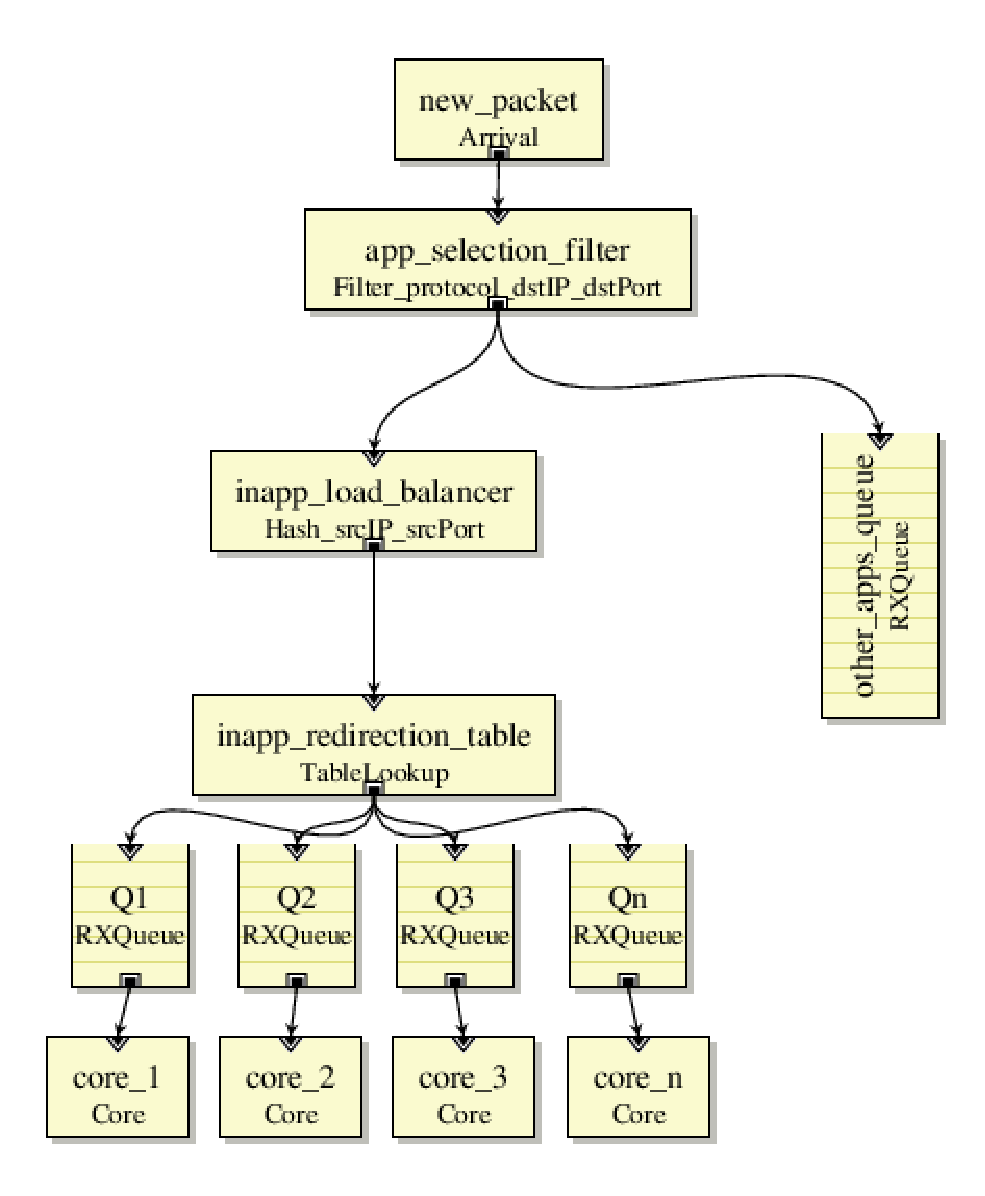
\includegraphics[width=0.5\textwidth]{figures/DNSServerIdeal.eps}
\caption{Ideal configuration for DNS server}
\end{figure*}


\begin{enumerate}
    \item One dedicated RX queue for each load balancing core.
    \item Hardware filter for (protocol, destination IP, destination port) to separate
    packets for this particular application.
    \item Ideal : Give each separated packet to next core in round-robin fashion
\end{enumerate}

\subsubsection{Alternate setup: 1}
\begin{enumerate}
       \item Hash (source ip, source port) (assuming uniform distribution of hash values)
       \item Use hash to select one of the dedicated RX queues.
\end{enumerate}

\subsubsection{Alternate setup: 2}
\begin{enumerate}
       \item Use one RX queue and one filter (protocol, destination IP,
        destination port) for this application, and let all the cores
        share the same RX queue.
        (not a good idea due to contention on updating RX)
\end{enumerate}

--------------------------------
\subsection{Application:  HTTP server (eg: apache)}
A server responding with small sized static pages
\subsubsection{Requirements:}
\begin{enumerate}
    \item TCP protocol
    \item Single listen port
    \item Preference to throughput
    \item Large number of incoming clients
    \item Small request, larger response.
    \item Load balancing with multiple cores
\end{enumerate}

\subsubsection{Ideal hardware setup}

\begin{figure*}[t]
\centering
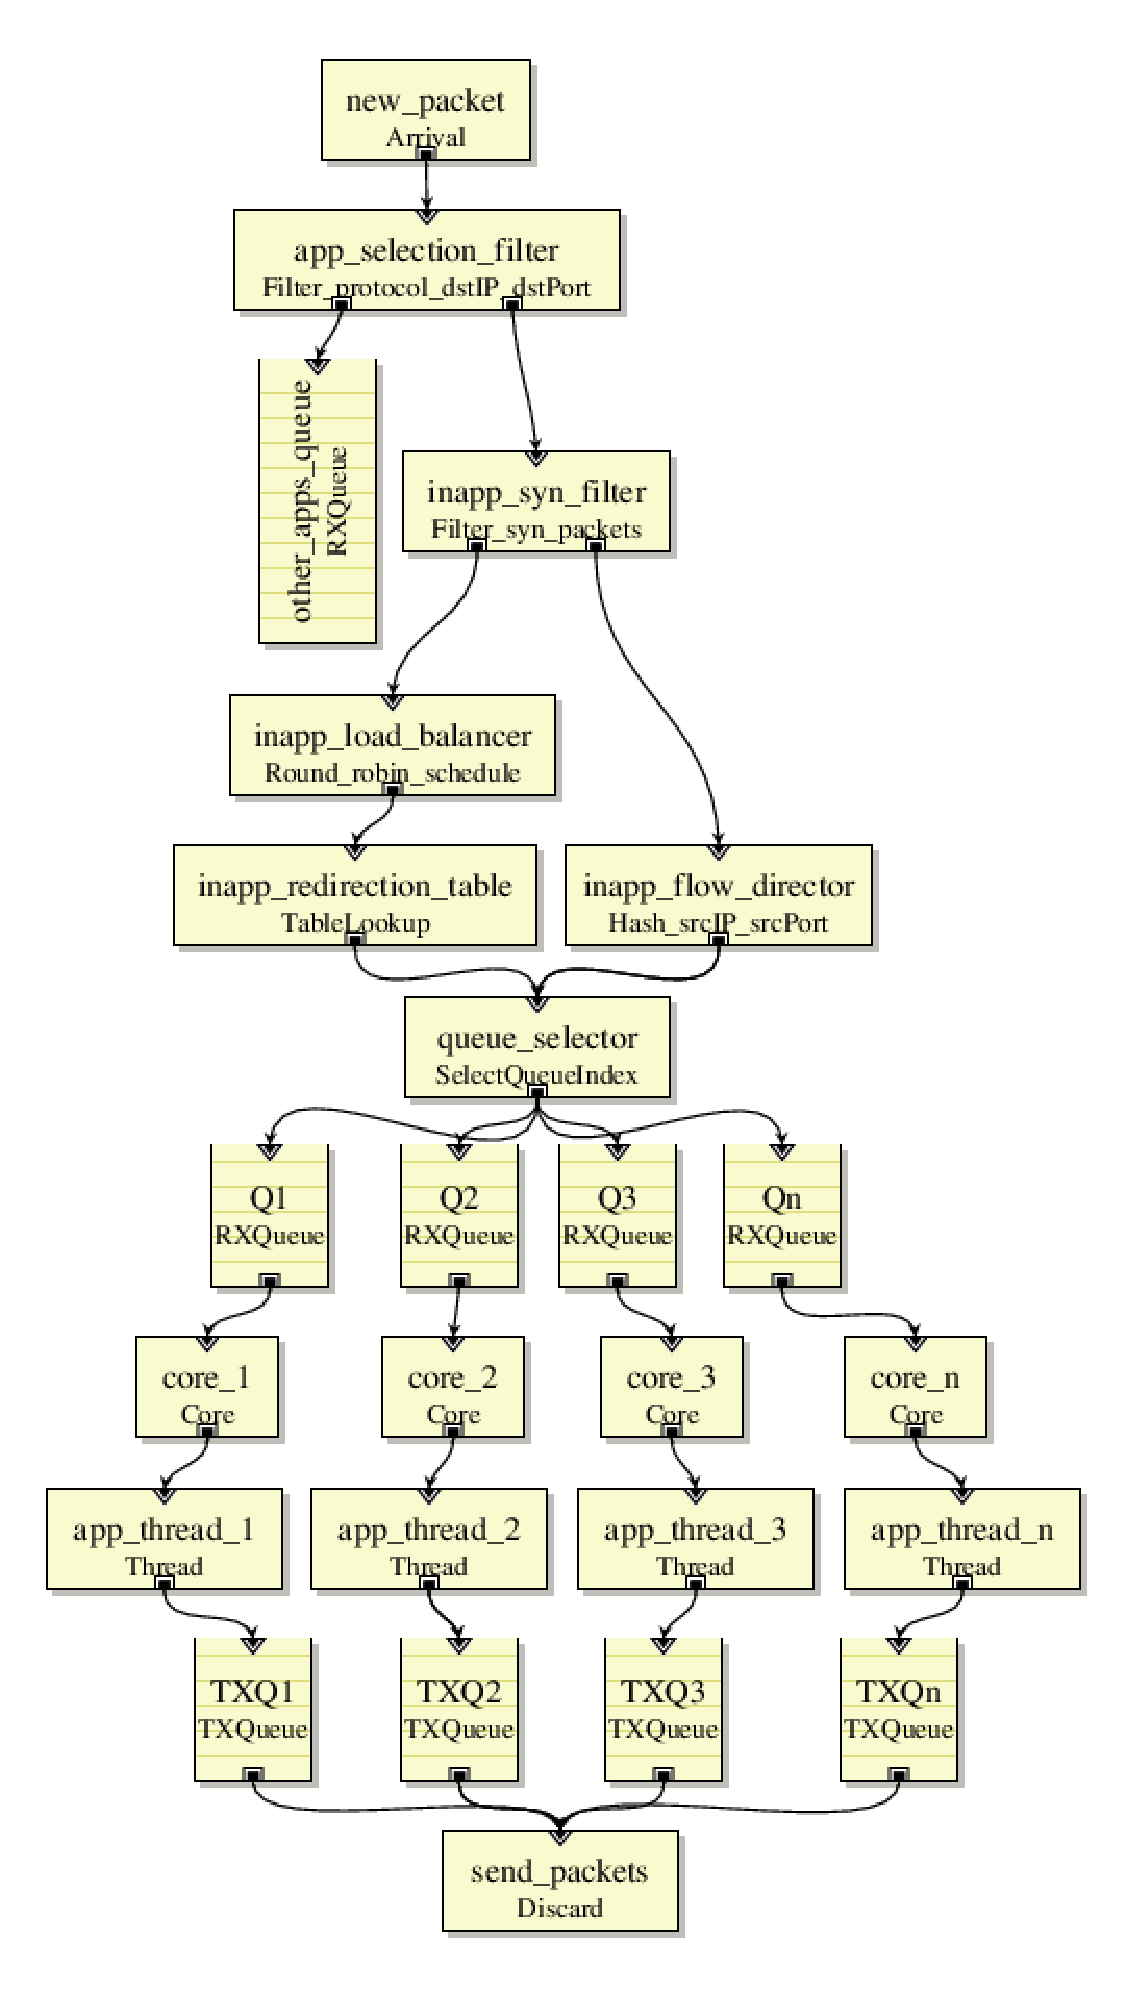
\includegraphics[width=0.5\textwidth]{figures/HTTPServerIdeal.eps}
\caption{Ideal configuration for HTTP server}
\end{figure*}

\begin{enumerate}
    \item One dedicated RX queue for each load balancing core.
    \item Hardware filter for (protocol, destination IP, destination port)
    \item Ideal : Give each new connection to next core in round-robin fashion
\end{enumerate}

\subsubsection{Alternate setup: 1}
\begin{enumerate}
       \item Hash (source ip, source port)
       \item Use hash to select one of the dedicated RX queues.
\end{enumerate}

\subsubsection{Alternate setup: 2}
\begin{enumerate}
       \item Use syn filter to separate syn packets
       \item Give all syn packets to load balancer
       \item Load balancer will distribute them in round-robin manner
       \item Insert new flow directing filter to ensure rest of the packet of
        this connection goes directly to proper core.
\end{enumerate}


\subsection{Application: Web crawler}

\subsubsection{Requirements:}
\begin{enumerate}
    \item HTTP/TCP Protocol
    \item Large number of outgoing connections
    \item Large incoming data
    \item Relatively small connection lifetime (HTTP requests)
    \item Scale by adding more cores running same application with different
        targets
    \item Preference to throughput
\end{enumerate}
%\todo{Complete the requirements of this application}

\subsubsection{Ideal hardware setup}

\begin{figure*}[t]
\centering
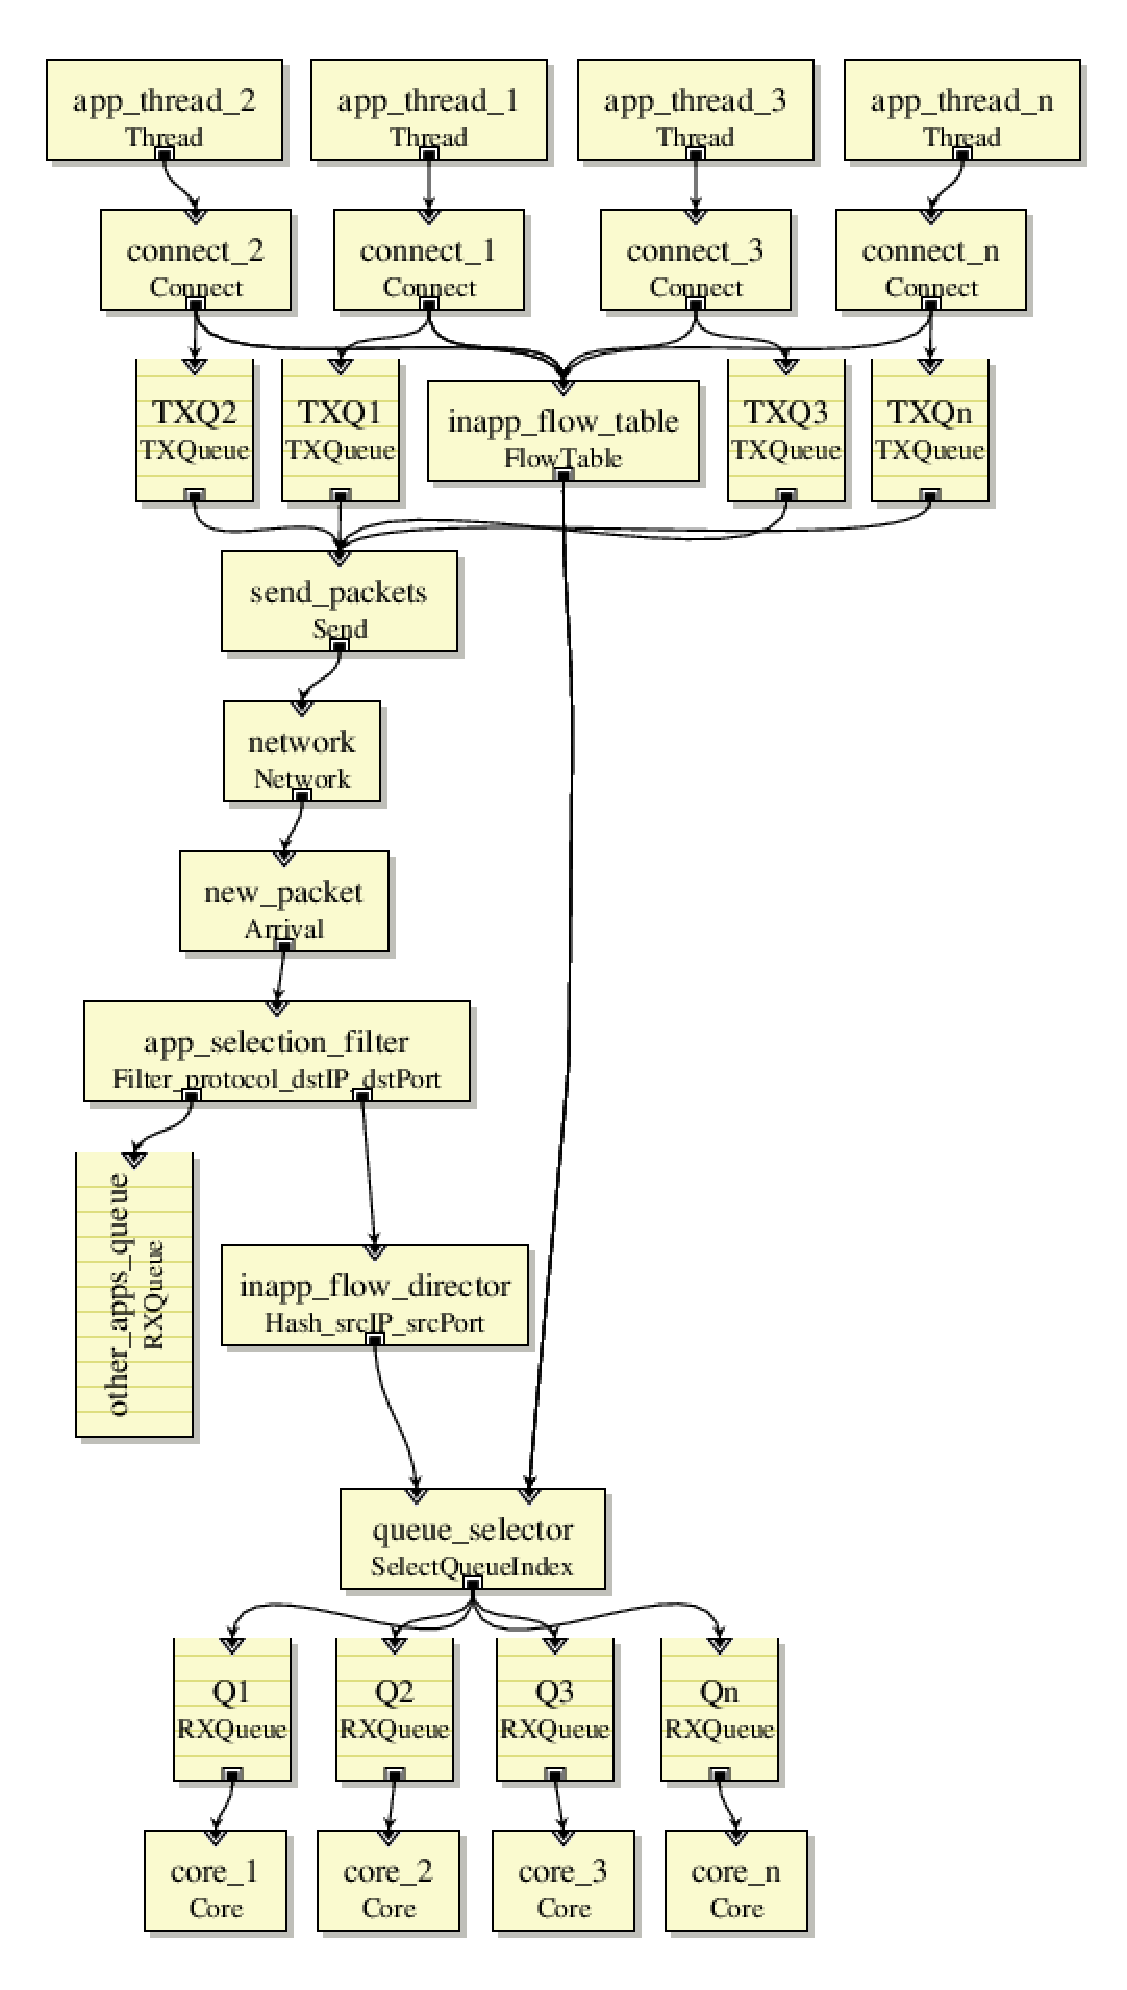
\includegraphics[width=0.5\textwidth]{figures/WebCrawlerIdeal.eps}
\caption{Ideal configuration for Web crawler}
\end{figure*}

\begin{enumerate}
    \item A dedicated RX queue for every core involved in load-balancing
    \item A dedicated hardware filter for every outgoing connection
    \item Filtering based on $(protocol, src-ip, src-port,  dest-IP, dest-port)$
    \item Dedicated queue for each load-balancing core
\end{enumerate}

\subsection{Application: Web Proxy}

\subsubsection{Requirements:}
\begin{enumerate}
    \item HTTP/TCP Protocol
    \item Single listen port
    \item Large number of incoming connections
    \item Large number of outgoing connections
    \item Relatively small connection lifetime for outgoing connections.
    \item Larger connection lifetime for incoming connections (client connections)
    \item Scaling??
    \item Preference to latency and throughput (not sure)
    \item With high probability, Incoming and outgoing connections are on
            different interfaces
    \item Examples: Squid
\end{enumerate}

\subsubsection{Ideal hardware setup}
\begin{enumerate}
    \item One dedicated hardware filter for incoming connections
    \item Filtering based on (protocol, destination IP, destination port)
    \item Hashing to load balance connections hash(source IP, source port)
    \item Dedicated queue for each load-balancing core
    \item Distribution of connections across cores in round-robin fashion.
    \item Does not make much sense to have a dedicated queues for outgoing
            connections.
\end{enumerate}



\subsection{Application: NFS filesystem client}
A kernel code which connects to NFS server and gets the contents of files
based on application requests.
\subsubsection{Requirements:}
\begin{enumerate}
    \item UDP protocol
    \item Single connect port (outgoing connection)
    \item Preference to throughput
    \item Small request, large response. (reading data)
    \item Load balancing: Increase number of kernel threads doing IO over NFS.
        The queries and responses are marked by RPC transaction-IDs which
        can be used to map the responses to proper kernel thread.
\end{enumerate}



\subsubsection{Ideal hardware setup}
\begin{enumerate}
    \item One dedicated RX queue for each load balancing core.
    \item Hardware filter for (protocol, destination IP, destination port)
    \item Give each packet to proper kernel thread based on RPC
        transaction ID.
\end{enumerate}

\subsubsection{Alternate setup: 1}
If there is only one application
\begin{enumerate}
    \item Use hash(source IP, source port) to select the destination core.
\end{enumerate}





\subsection{Application: MPI application}
A class of scientific applications which communicate with each other using
runtimes like MPI and perform some computation in distributed fashion.


\subsubsection{Requirements:}
\begin{enumerate}
    \item TCP Protocol
    \item Small messages
    \item Large number of messages
    \item Preference to low latency
    \item Scalability with number of nodes
    \item Long connection lifetime. (Assuming all messages are using same
            channel established once per node)
\end{enumerate}

\subsubsection{Ideal hardware setup}
\begin{enumerate}
    \item How many filters?
\end{enumerate}


\subsection{Application:  Database server (eg: mysql!!)}
A server handling small number of clients with large number of queries
\subsubsection{Requirements:}
\begin{enumerate}
    \item TCP protocol
    \item Single listen port
    \item Preference to throughput
    \item small number of incoming clients
    \item Small request, large response.
    \item Load balancing with ??
  %  \todo{Not complete and useful yet!, get more accurate data about this setup}
\end{enumerate}



\subsection{Application: Firewall}

\subsubsection{Requirements:}
\begin{enumerate}
    \item Protocol??
\end{enumerate}

\subsubsection{Ideal hardware setup}
\begin{enumerate}
    \item How many filters?
\end{enumerate}

\subsection{Application: Intrusion Detection System }

\subsubsection{Requirements:}
\begin{enumerate}
    \item Protocol??
\end{enumerate}

\subsubsection{Ideal hardware setup}
\begin{enumerate}
    \item How many filters?
\end{enumerate}




\subsection{Application: }

\subsubsection{Requirements:}
\begin{enumerate}
    \item Protocol??
\end{enumerate}

\subsubsection{Ideal hardware setup}
\begin{enumerate}
    \item How many filters?
\end{enumerate}



\subsection{Application: }

\subsubsection{Requirements:}
\begin{enumerate}
    \item Protocol??
\end{enumerate}

\subsubsection{Ideal hardware setup}
\begin{enumerate}
    \item How many filters?
\end{enumerate}



%\section{test diagrams}

\pagebreak

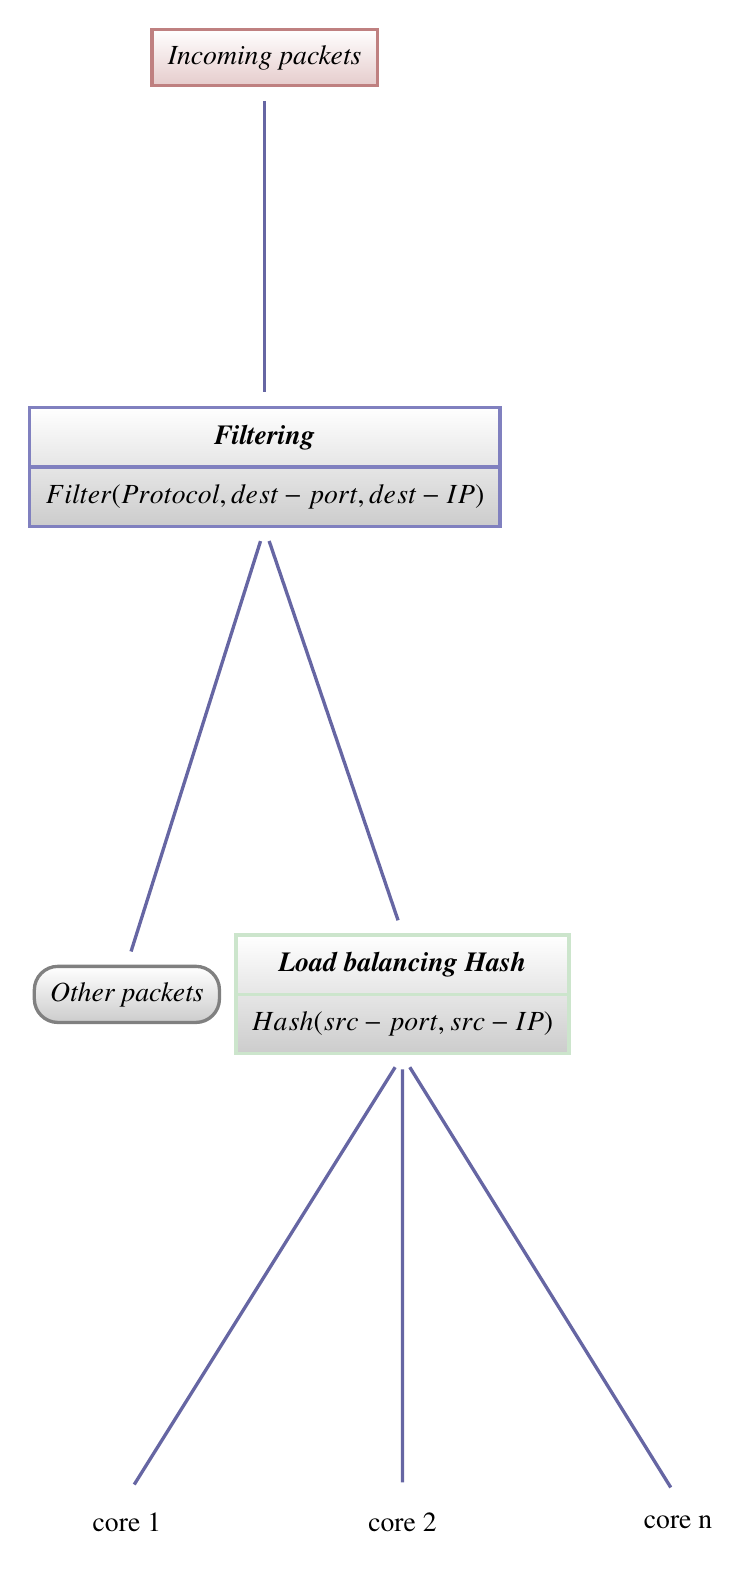
\begin{tikzpicture}[
    grow=down,
    level 1/.style={sibling distance=3.5cm,level distance=5.2cm},
    level 2/.style={sibling distance=3.5cm, level distance=6.7cm},
    edge from parent/.style={very thick,draw=blue!40!black!60,
        shorten >=5pt, shorten <=5pt},
    edge from parent path={(\tikzparentnode.south) -- (\tikzchildnode.north)},
    kant/.style={text width=2cm, text centered, sloped},
    every node/.style={text ragged, inner sep=2mm},
    incomingp/.style={rectangle, minimum size=6mm, very thick,
        draw=red!50!black!50, top color=white, bottom color=red!50!black!20,
        font=\itshape},
    QueueShape/.style={rectangle, minimum size=6mm, rounded corners=3mm,
        very thick, draw=black!50, top color=white, bottom color=black!20,
        font=\itshape},
    FilterShape/.style={rectangle, minimum size=6mm, very thick,
        draw=blue!50!black!50, top color=white, bottom color=black!20,
        font=\itshape},
    HashShape/.style={rectangle, minimum size=6mm, very thick,
        draw=green!50!black!20, top color=white, bottom color=black!20,
        font=\itshape}
]
\node (incoming) [incomingp] {Incoming packets}
    child {
        node (filter1) [FilterShape] [rectangle split, rectangle split,
            rectangle split parts=2, text ragged] {
            \textbf{Filtering}
                  \nodepart{second}
            $ Filter(Protocol, dest-port, dest-IP) $
            }
            child { node (otherPackets) [QueueShape] {Other packets}}
            child {
                node (hash1) [HashShape] [rectangle split, rectangle split,
                    rectangle split parts=2, text ragged] {
                    \textbf{Load balancing Hash}
                        \nodepart{second}
                   $ Hash(src-port, src-IP) $
                    }
                    child {node {core 1}}
                    child {node {core 2}}
                    child {node {core n}}
                    }
    };
\end{tikzpicture}

\pagebreak


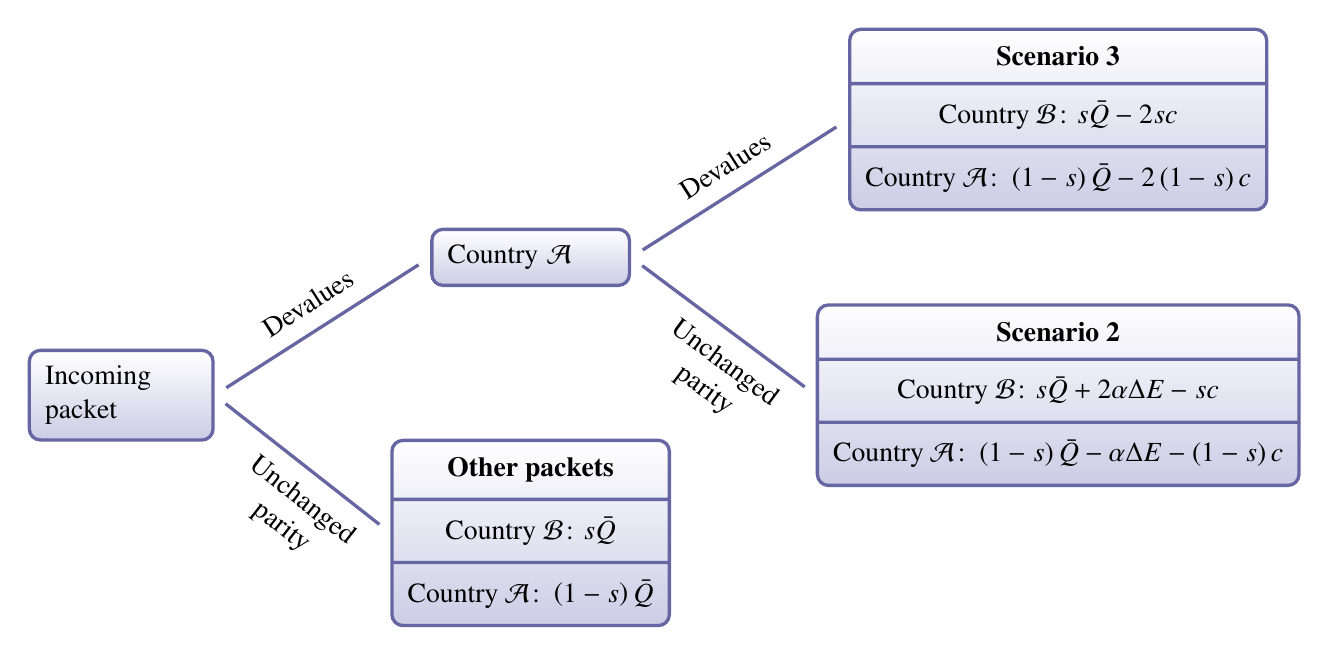
\begin{tikzpicture}[
    grow=right,
    level 1/.style={sibling distance=3.5cm,level distance=5.2cm},
    level 2/.style={sibling distance=3.5cm, level distance=6.7cm},
    edge from parent/.style={very thick,draw=blue!40!black!60,
        shorten >=5pt, shorten <=5pt},
    edge from parent path={(\tikzparentnode.east) -- (\tikzchildnode.west)},
    kant/.style={text width=2cm, text centered, sloped},
    every node/.style={text ragged, inner sep=2mm},
    punkt/.style={rectangle, rounded corners, shade, top color=white,
    bottom color=blue!50!black!20, draw=blue!40!black!60, very
    thick }
    ]


\node[punkt, text width=5.5em] {Incoming packet}
    %Lower part lv1
    child {
        node[punkt] [rectangle split, rectangle split, rectangle split parts=3,
         text ragged] {
            \textbf{Other packets}
                  \nodepart{second}
            $\text{Country \B}\colon    s\bar{Q}$
                  \nodepart{third}
            $\text{Country \A}\colon\pa{1-s}\bar{Q}$
        }
        edge from parent
            node[kant, below, pos=.6] {Unchanged parity}
    }
    %Upper part, lv1
    child {
        node[punkt, text width=6em] {Country~\A}
        %child 1
        child {
            node [punkt,rectangle split, rectangle split,
            rectangle split parts=3] {
                \textbf{Scenario  2}
                \nodepart{second}
                $\text{Country \B}\colon s\bar{Q}+2\alpha\Delta E -sc$
                \nodepart{third}
                $\text{Country \A}\colon\pa{1-s}\bar{Q}-\alpha\Delta E -
                \pa{1-s}c$
            }
            edge from parent
                node[below, kant,  pos=.6] {Unchanged parity}
        }
        %child 2
        child {
            node [punkt, rectangle split, rectangle split parts=3]{
                \textbf{Scenario 3}
                \nodepart{second}
                $\text{Country \B}\colon s\bar{Q}-2sc$
                \nodepart{third}
                $\text{Country \A}\colon\pa{1-s}\bar{Q}-2\pa{1-s}c$
            }
            edge from parent
                node[kant, above] {Devalues}}
            edge from parent{
                node[kant, above] {Devalues}}
    };
\end{tikzpicture}




% % % % % % % % % % % % % % % % % % % % % % % % % % % % % % % % % % % %
%test citation ~\cite{barrelfish}

%{\footnotesize
\bibliography{workloadRefs}
\bibliographystyle{acm}
%}

\end{document}

